\chapter{Transformation}% by Mugdho Tanjim Shorif}

\begin{linkb}
   \begin{itemize}
        \item  \href{https://www.youtube.com/watch?v=yohxAxqnCt8}{Video 1}, \href{https://www.youtube.com/watch?v=7tAmJ8cvmYM}{Video 2}
        \item \href{https://drive.google.com/file/d/1_XBfSBLO3NSWAKw9_mkhYPIWgkRfwm2Z/view}{(Boby Poon) } + \href{https://drive.google.com/file/d/11kMt5af6pfZDoaV932MsEf6Sx0vvznsk/view}{The Real Big Picture}
   \end{itemize}
\end{linkb}


There are generally  5 kind of Transformation, namely:
\begin{itemize}
	\item Translation
	\item Rotation
	\item Reflection
	\item Homothety
	\item Spiral Similarity		
\end{itemize}

\section{Translation}
This is the most common  and easy of the transformations, you can translate a point along with a line. Let the point is $P$ and the line is $AB$, then if you translate $P$ wrt $AB$, we write this as $T(AB)$ and here $P$ maps to a point $Q$ such that $AB \parallel PQ, $ and $AB=PQ$.

\begin{figure}[ht]
\centering
	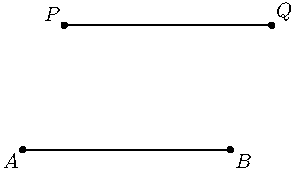
\includegraphics{translate1.pdf}
	\caption{Translation along with $AB$ maps $P$ to $Q$.}
\end{figure}

Here we are going to solve some problem.
\begin{example}
In the figure below, what is the minimal distance from $A$ to $B$ with a bridge that can be made in anywhere over the river perpendicular to the parallel lines.
\end{example}

\begin{figure}[ht]
\centering
		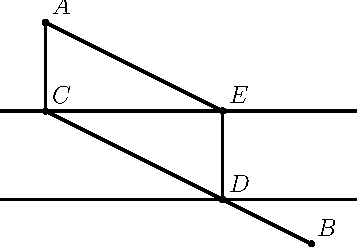
\includegraphics{translate2.pdf}
	\caption{Find shortest path from $A$ to $B$.}
\end{figure}

\begin{problem}
Similarly above find the shrtest distance from $A$ to $B$ with more that one river between them.
\end{problem}

\begin{example}
Let $ABCDEF$ be a hexagon such that, $AB\parallel DE, BC \parallel EF, CD \parallel FA$ and $AF-CD=DE-AB = BC -EF >0$. Prove that the hexagon is equiangular that is all the angles of the hexagon is equal  to $120\dg$.
\end{example}

\begin{figure}[ht]
\centering
	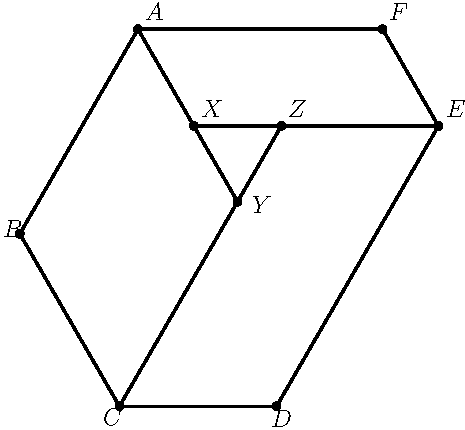
\includegraphics{translate3.pdf}
	\caption{Finding an equilateral triangle}
\end{figure}

Here the opposite sides configuration is very disgusting to handle. So we want such a translation which makes the subtraction of th opposite sides to the side of an equilateral triangle. We are going to translate $E$ along with $AF$ to map $E$ to $X$, similarly define $Y,Z$. Now observe that $XYZ$ is an equilateral triangle. Now it is easy to conclude.


\begin{example}
In quadrilateral $ABCD$, let $M,N$ be the midpoints of $AB$ and $CD$ respectively. Given that, $@MN=AD+BC$. Prove that, $AD\parallel BC$. 
\end{example}

%--------
\section{Rotation}
Rotation deals with a center point and an angle. Let a point be $P$ and another center point $O$. You may rotate $P$ wrt $O$ with angle $50\dg$ which means you draw an arc with center $O$ and goes from $P$ to $Q$.
And $\angle POQ =50\dg$.
It is defined by \[R(O,\alpha)\]
\begin{example}
Let, $ABCD$ be a square and $P$ be a point inside the square such that, $PA=1, PB=2, PC=3$. Find $\angle APB$.
\end{example}

Here we are going to rotate the points $A,C,P$ with center $B$ and angle of $90\dg$. Which means $A\mapsto C, P\mapsto P'$. Now note that as $\angle PBP'=90\dg$ and $PB=BP'$, we have, $\angle BPP'=45\dg=BP'P$. By Pythagoras, $PP'=2\sqrt 2$. As $AP =CP'=1$,  by the converse of Pythagoras we have, $\angle PP'C =90\dg$. So $\angle APB = \angle CP'B =90\dg$.

\begin{example}
Let $ABC$ be an equilateral triangle and a point inside the triangle $P$ such that $PA=5, PB=4, PC=3$. Find the area of the triangle.
\end{example}
\begin{figure}[ht]
\centering
		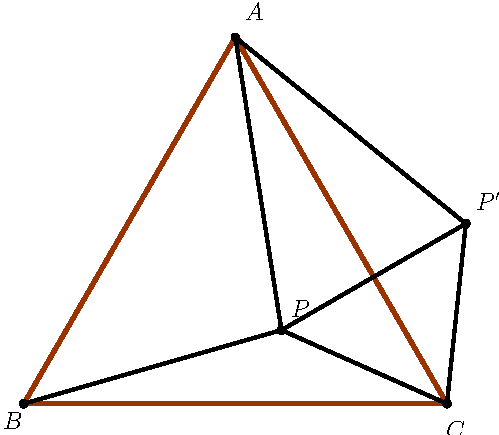
\includegraphics{rotate1.pdf}
	\caption{Rotate the point $P$}
\end{figure}
Consider a rotation with center $C$ and angle $60\dg$, $P\mapsto P', B\mapsto A$ and see that, \[CP'=CP\]
\[CA=CB\]
\[\angle P'CA = \angle PCB\]
Here you see that, \[AP'=BP=4\]
\[PP'=3\]
and $APP'$ is a right angular triangle with $\angle AP'P=90\dg$.
So, \[ \angle AP'C=150\dg=\angle BPC \]
By cosine law we are done!


\begin{example}
Let $ABCD$ be a square and $W,X,Y,Z$ be four points on $AB,BC,CD,DA$ respectively such that $BW+BX+DY+DZ=2BC$. Prove that, $WY\perp ZX$. 
\end{example}
Here rotate the diagram with center $B$ and
 angle $90\dg$. We denote the rotation of $A$
  with $A'$ and analogous...


AND we are giong to show that $WY \parallel Z'X'$
\begin{figure}[ht]
\centering
		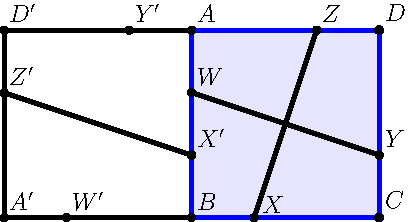
\includegraphics{rotate2.pdf}
	\caption{Perpendicularity to Parallelism!}
\end{figure}
Here we let $AB=BC=CD=DA=a$.
And doing some calculation:
\begin{align*}
BW+BX+DY+DZ &=2BC=2a\\
BW'+BX+D'Y'+DZ &=2a\\
BW'+BX+(a-AY')+(a-AZ) &=2a\\
BW'+BX &= AY'+AZ\\
XW'&=Y'Z
\end{align*}
Now it is easy to see that $XZY'W'$ is a parallelogram. And that's why $ZX\parallel W'Y'$.
%------------
\section{Reflection}

\begin{example}
Let $ABCD$ be a quadrilateral such that, $AB=BC=CD$ and $AC \neq BD$ but $AE=DE$ where $E$ is the intersection of the diagonals. Find $\angle BAD + \angle ADC$.
\end{example}

\begin{figure}
\centering
	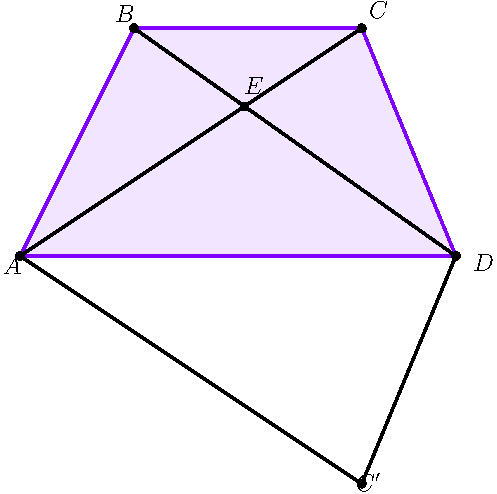
\includegraphics{reflection1.pdf}
 	\caption{A reflection problem}
 \end{figure}
Here we are goingt to reflect $C$ with respect to $AD$ and we get that $BD\parallel AC'$ and $C'D=AB$. SO $ABDC'$ is either a parallelogram or trapezoid. 

But there is a contradiction that if it is a paralleogram then $AC'=AC=BD$ which is absurd.

So it is an isosceles trapezoid which is obviously cyclic.
Here we denote $\angle BAC=\beta=\angle BCA$, $\angle CAD =\angle DAC'=\angle BDA=\alpha$, $\angle DBC=\gamma$.

So we get $\angle ADC'=\alpha +\gamma $
Using cyclic quads, we get $4\alpha=120\dg$. (Yes, there is some angle chasing which is a good exercise and left to the reader.)

Here is a problem you can try:
\begin{problem}
A circle with center $O$ passes through vertices $A$ and $C$ of $\triangle ABC$ and cuts sides $AB,BC,CA$ at $K$ and $N$ respectively. The circumcircles of $ABC$ and $KBN$ intersect at $B$ and $M$. Prove that $\angle OMB=90\dg$.
\end{problem}

\section{Homothety}
Homothety (also known as dilation) is a 
transformation consisting of two variables- 
a center $O$ and a real number $k$ such that
$O$ sends a point $A$ to $A'$.
Homothety is denoted by-
\[ H(O, k)\]
Remember that $k$ can be negative

We have, \[ \frac{OA'}{OA}=k.\]

\begin{enumerate}
	\item After homothety $AB$ and $A'B'$ are parallel.
	\item Triangles are similar after homothety.
	%\item
\end{enumerate}
See the diagram. Here $O$ sends $A, B, C$ to $h(A), h(B), h(C)$ respectively.

\begin{figure}[ht]
\centering
	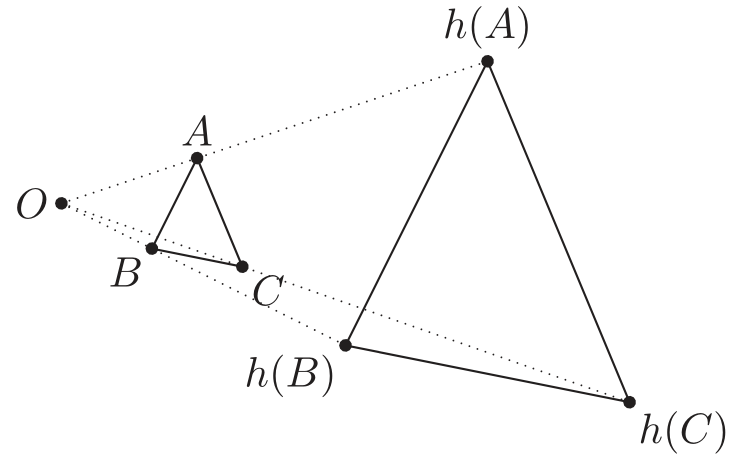
\includegraphics[scale=0.3]{homothety.png}
	\caption{$\triangle ABC$ and $\triangle  h(A), h(B), h(C)$ are homothetic similar}
\end{figure}
As said before $k$ can be negative. See the diagram-

\begin{figure}[ht]
\centering
	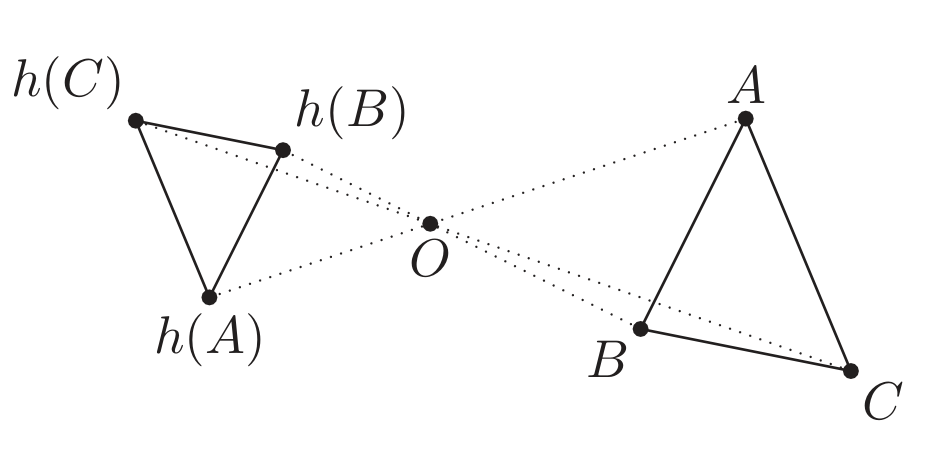
\includegraphics[scale=0.3]{neg-homothety.png}
	\caption{A negative homothety}
\end{figure}
Also remember that homothetic center can be a point at infinity. Where $AB=A'B'$ and the scale factor of the homothety is not equal to $-1$.



\begin{example}
Two circles $C_1, C_2$ are such that $C_2$ is internally tangent  to $C_1$ at $P$. A chord $AB$ of $C_1$ touches $C_2$ at $E$. Prove that ray $PE$ bisects the arc $AB$ which doesn't contains $P$.
\end{example}

We are going to use homothety here. Look
 that $P$ is the homothetic center of two 
 circles that sends $C_2$ to $C_1$.
Let $O_1, O_2$ vare the centers of $C_1, C_2$ respectively, see that $P,O_1,O_2$ are collinear.
Also $P,E,F$ (where $F$ is the intersection point of $PE$ with $C_1$) are collinear. Consequently $PO_2E$ and $PO_1F$ are homothetic. Here note that $\angle O_2EA=90\dg$ similarly $F$ is the tangent point of a line parallel to $BA$ whch is tangent to $C_1$. 

Here we see a proof of the nine point circle.
\begin{figure}[H]
\centering
	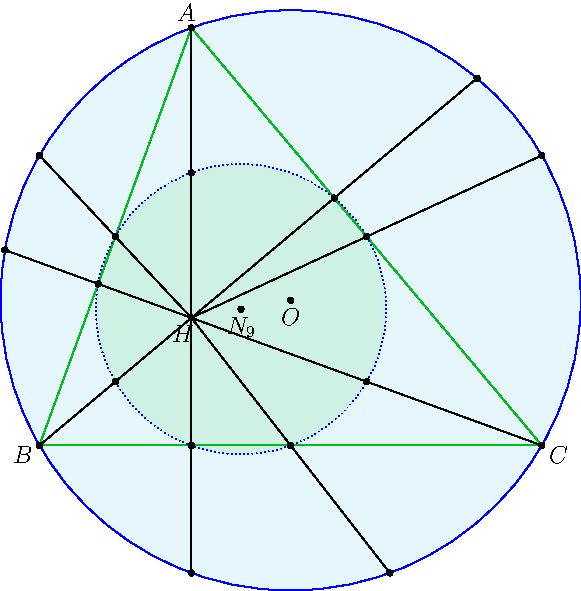
\includegraphics{npc-homo.pdf}%[scale=0.3]{npc.png}
	\caption{Nine Point Circle Homothetic to $(ABC)$ with center $H$.}
\end{figure}
You probably know the fact that the reflection of the orthocenter on the line $BC$ and with respect to the midpoint of $BC$ lies on the circumcircle of $ABC$.
Similarly, define analogous points.
Here you get nine points on the circumcircle of $ABC$. Consider a homothety with center $H$ and scale factor $\half$. So we get nine points still concyclic. Done!

\begin{problem}\label{prob:homo}
Let the incircle of triangle $ABC$ touches $BC$ at $D$. $T$ is the antipode of $D$ with respect to the incircle. Let ray $AT$ meets $BC$ at $P$. Prove that $BD=CP.$
\end{problem}


\begin{figure}[ht]
\centering
	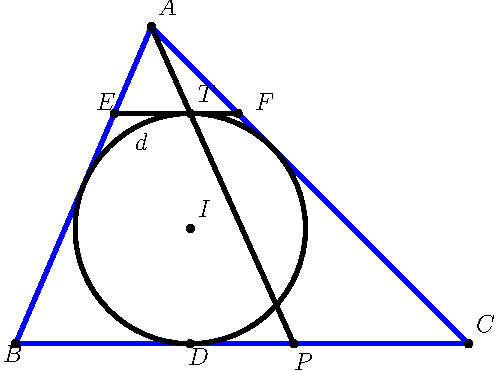
\includegraphics{homo-prob.pdf}
	\caption{\autoref{prob:homo} for exercise}
\end{figure}

\section{Spiral Similarity}
Spiral similarity isa special kind of similarity consisiting of a rotation and a dilation(homothety). It is denoted by \[S (O,\alpha ,k)\] where $O$ is the center of the spiral similarity.
%or denoted by S 

\begin{example}
$P$ is an internal point in the plane of a triangle $ABC$ such that $\angle APC=\angle BPC=\angle APB=120\dg$ and $\angle BAC =60\dg$. Let, $D,E$ be the midpoints of the segments $AC,AB$ respectively. Show that $AEPD$ cyclic.
\end{example}
\begin{figure}[ht]
\centering
	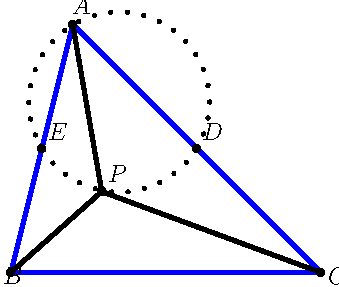
\includegraphics{spiral1.pdf}
	\caption{A spiral similarity problem}
\end{figure}
Here see that $\triangle APB$ and $\triangle CPA$ aer similar.
So we can take a spiral similarity that takes $APB$ to $CPA$ with center $P$ and angle $120\dg$.
\[S(P,120\dg,\frac{PC}{PA})\]
\[A\mapsto C\]
\[B\mapsto A\]
So we can say that \[E\mapsto D.\]
So, as our angle of rotation was $120\dg$ so $\angle EPD=120\dg=180\dg - \angle EAD.$
Done!

%And class ends here!






